% Template for Cogsci submission with R Markdown

% Stuff changed from original Markdown PLOS Template
\documentclass[10pt, letterpaper]{article}

\usepackage{cogsci}
\usepackage{pslatex}
\usepackage{float}
\usepackage{caption}

% amsmath package, useful for mathematical formulas
\usepackage{amsmath}

% amssymb package, useful for mathematical symbols
\usepackage{amssymb}

% hyperref package, useful for hyperlinks
\usepackage{hyperref}

% graphicx package, useful for including eps and pdf graphics
% include graphics with the command \includegraphics
\usepackage{graphicx}

% Sweave(-like)
\usepackage{fancyvrb}
\DefineVerbatimEnvironment{Sinput}{Verbatim}{fontshape=sl}
\DefineVerbatimEnvironment{Soutput}{Verbatim}{}
\DefineVerbatimEnvironment{Scode}{Verbatim}{fontshape=sl}
\newenvironment{Schunk}{}{}
\DefineVerbatimEnvironment{Code}{Verbatim}{}
\DefineVerbatimEnvironment{CodeInput}{Verbatim}{fontshape=sl}
\DefineVerbatimEnvironment{CodeOutput}{Verbatim}{}
\newenvironment{CodeChunk}{}{}

% cite package, to clean up citations in the main text. Do not remove.
\usepackage{apacite}

% KM added 1/4/18 to allow control of blind submission


\usepackage{color}

% Use doublespacing - comment out for single spacing
%\usepackage{setspace}
%\doublespacing


% % Text layout
% \topmargin 0.0cm
% \oddsidemargin 0.5cm
% \evensidemargin 0.5cm
% \textwidth 16cm
% \textheight 21cm

\title{Sticks, leaves, bowls, and buckets: Distributional patterns of
children's at-home object handling in two subsistence societies}

\usepackage{booktabs}
\usepackage{longtable}
\usepackage{array}
\usepackage{multirow}
\usepackage{wrapfig}
\usepackage{float}
\usepackage{colortbl}
\usepackage{pdflscape}
\usepackage{tabu}
\usepackage{threeparttable}
\usepackage{threeparttablex}
\usepackage[normalem]{ulem}
\usepackage{makecell}
\usepackage{xcolor}

\author{Kennedy Casey \\
        University of Chicago \\
        \texttt{\small{kbcasey@uchicago.edu}}
\And \textbf{Mary Elliott} \\
             University of Texas at Dallas \\
             \texttt{\small{maryle18@gmail.com}}
\And \textbf{Anapaula Silva Mandujano} \\
             University of Chicago \\
             \texttt{\small{anapaula@uchicago.edu}}   
\And \textbf{Kimberly Shorter} \\
             University of Chicago \\
             \texttt{\small{klshorter@uchicago.edu}}
\AND \textbf{Elizabeth Mickiewicz} \\
             University of Chicago \\
             \texttt{\small{lizmick9@uchicago.edu}}         
\And \textbf{Mara Duquette} \\
             University of Chicago \\
             \texttt{\small{duquettemara@uchicago.edu}}
\And \textbf{Elika Bergelson} \\
             Duke University \\
             \texttt{\small{elika.bergelson@duke.edu}}
\And \textbf{Marisa Casillas} \\
             University of Chicago \\
             \texttt{\small{mcasillas@uchicago.edu}}}

\newlength{\cslhangindent}
\setlength{\cslhangindent}{1.5em}
\newenvironment{CSLReferences}%
  {}%
  {\par}

\begin{document}

\maketitle

\begin{abstract}


\textbf{Keywords:}

\end{abstract}

\hypertarget{introduction}{%
\section{Introduction}\label{introduction}}

The artifacts of everyday life reflect our routines, aspirations,
relationships, and more. In particular, the objects that we regularly
pick up and handle---a coffee cup, a laptop, a baby bottle---offer a
window into the physical, social, and cultural contexts that shape our
understanding of the world. In this paper, we take a glimpse into
everyday life at its beginnings by exploring children's at-home object
handling from early infancy until age four. We contextualize our study
with respect to the effects of object-centric interaction on word
learning, though we note that different analyses of these same data
could shed new light on other types of social learning as well as motor
development (see Herzberg, Fletcher, Schatz, \& Tamis-LeMonda, 2021, on
the latter point).

\hypertarget{object-handling-and-word-learning}{%
\subsection{Object handling and word
learning}\label{object-handling-and-word-learning}}

For young learners, objects---along with their associated activities and
surrounding language---form a critical source of input for word
learning. Hands (and what they are handling) can be reliable indicators
of what someone is doing and talking about during object play and can
thus help learners map word forms onto their meanings in and across
real-time interaction (e.g., Yu \& Smith, 2013; Yurovsky, Smith, \& Yu,
2013). Present, attended-to objects also influence the babble of
children who have acquired stable consonants (Laing \& Bergelson, 2020).
Further, caregivers' tendency to use nouns referring to objects in the
here-and-now positively predicts their children's early word
comprehension (Bergelson \& Aslin, 2017).

How frequently do children engage in object-centric interactions? First,
hands---others' and their own---are in good supply in young children's
view of the world, especially after early infancy (Fausey, Jayaraman, \&
Smith, 2016; Jayaraman, Fausey, \& Smith, 2017; Long, Kachergis,
Agrawal, \& Frank, 2020). Infants' own object handling is also
relatively frequent: Herzberg and colleagues (2021) find that US infants
handle objects \(\sim\) 60\% of the time during at-home play, Yu and
colleagues (2013) find \(\sim\) 70\% when including joint handling with
adults in US in-lab object play, and Casillas and Elliott (2021) find
\(\sim\) 15 and 17\% object handling in daylong photo streams in a
Papuan and a Mayan community, respectively. Note, however, that
\emph{labeling} of object-relevant features (e.g., names and associated
concepts) is the critical second ingredient for word learning, which may
only occur during a small subset of total object handling time.
Additionally, the likelihood of talk about objects that are being
handled in the here and now---a flagship feature of contingent caregiver
talk (e.g., McGillion et al., 2013)---fluctuates across high and low
activity periods of interaction (Bergelson, Amatuni, Dailey, Koorathota,
\& Tor, 2019).

Overall, while prior work makes a strong case for the impact of
children's object-centric interactions on their word learning, the
findings: (a) are limited to a culturally narrow sample of populations,
(b) have tended to rely on short recordings that limit the scope of
object-centered interactions analyzed, and (c) have rarely examined in
detail the distributions of individual objects that children typically
interact with at home (exceptions include Bergelson, Amatuni, Dailey,
Koorathota, \& Tor, 2019; Casillas \& Elliott, 2021; Herzberg, Fletcher,
Schatz, \& Tamis-LeMonda, 2021).

\hypertarget{object-handling-across-age-and-culture}{%
\subsection{Object handling across age and
culture}\label{object-handling-across-age-and-culture}}

Children's object handling input changes enormously across the first few
years due to both maturational constraints and culture-specific
caregiving practices. In early infancy, children have little ability to
hold things or to control their posture, primarily experiencing objects
through what others bring near to them. Faces, rather than objects, may
make up a much greater proportion of their social input early on
(Fausey, Jayaraman, \& Smith, 2016; Jayaraman, Fausey, \& Smith, 2017;
but see also Long, Kachergis, Agrawal, \& Frank, 2020). However, later
gains in manual dexterity and gross motor skill (e.g., sitting,
crawling, walking) increasingly widen children's ability to seek, reach,
and grab a diversity of objects in their environment. Increasing motor
development not only gives children greater control over what objects
handle but also how they elicit social information relating to objects
and for how long (Adolph, Karasik, \& Tamis-LeMonda, 2010; Gaskins,
2000; Herzberg, Fletcher, Schatz, \& Tamis-LeMonda, 2021; Kretch,
Franchak, \& Adolph, 2014; Sanchez, Long, Kraus, \& Frank, 2018).

Early access to objects is also shaped by culture-specific practices for
carrying children, keeping them safe and warm, and scaffolding the
development of locally valued capacities (e.g., word learning in many US
families, walking in Kenyan Kipsigis families: Super, 1976; see Adolph,
Karasik, \& Tamis-LeMonda, 2010, for an overview). The array of objects
available to children will also vary in type and prevalence
cross-culturally. Objects spread via globalization (e.g., plastic bags)
and objects with a basic functional role that has arisen similarly
across many groups (e.g., spoon-like things for eating) are likely to
appear in widely, while other objects remain specific to people and
places (e.g., the gourd and bombilla for drinking mate in much of South
America, stemming from Indigenous Guaraní and Tupí tradition). Take, for
example, middle-class US family homes, which have been noted for their
large quantities of possessions (``clutter''), much of which is designed
specifically for children (e.g., toys and books, Arnold, Graesch, Ochs,
\& Ragazzini, 2012). We might infer, based on this distribution, that
much of what children do and talk about at home is tailored to what
particularly interests them. Thus, children's worlds, in this sense,
look very different from their caregivers'. Recent work by Herzberg and
colleagues (2021) underscores this point with infancy data; 13- to
23-month-olds spent nearly 70\% of their time in object play with toys
or a mix of toys and non-toys, with \(\sim\) 100\% of infants playing
with children's books and stuffed animals, and a total of 32 toy types
appearing in \(\ge\) 25\% of infants' play. Non-toy play was also
common, but still appeared to predominantly include infant-specific
objects (e.g., sippy cups, baby spoons, high chairs, pacifiers). We
would expect many of these items to be rare in other parts of the world,
with much greater overlap between objects for infants and objects for
adults (e.g., Karasik, Schneider, Kuchirko, \& Tamis-LeMonda, 2018).

\hypertarget{the-current-study}{%
\subsection{The current study}\label{the-current-study}}

Using daylong photo streams from child-worn cameras, we analyze object
handling by children under age four in two rural, small-scale
subsistence farming communities from opposite sides of the globe: Rossel
Island (``Rossel''; Milne Bay Province, Papua New Guinea) and Tenejapa
(``Tseltal''; Chiapas, Mexico). While these communities are comparable
in many ways (e.g., rural, swidden horticulturalist, housed in
multi-generation family complexes), prior work has established
substantial differences in the organization of young children's daily
lives, child carrying practices, and each community's level of market
integration (e.g., the greater availability of synthetic materials in
Tenejapa), leading us to expect differences in what children handle
across the day and early lifespan (Brown \& Casillas, 2021; Casillas,
Brown, \& Levinson, 2020, 2021; Casillas \& Elliott, 2021). We first
establish how often children handle objects from different categories
(e.g., food vs.~tools), both by the total amount of handling and by
number of unique objects per hour in each category across sites. We
explore the top individual objects in each site and how overlap exists
between sites. Finally, we investigate how the rate and characteristics
of object handling change with developmental age, as predicted in prior
work (Casillas \& Elliott, 2021).

Our findings reveal relative consistency in the broad composition of
objects handled by children, both between sites and across age, with a
few important exceptions: a greater diversity of synthetic objects per
hour for Tseltal children (e.g., relating to greater market
integration), more time spent with immovable objects for Rossel children
(e.g., relating to socializing time on/near household verandas), and a
greater diversity of held objects with developmental age. We discuss
open questions and potential implications of these findings for early
word learning.

\hypertarget{method}{%
\section{Method}\label{method}}

\hypertarget{corpus}{%
\subsection{Corpus}\label{corpus}}

Daylong photo streams consisted of images captured approximately every
15 (Rossel) to 30 (Tseltal) seconds over the course of 8 (Rossel) to 9
(Tseltal) waking hours at home. Children wore a recording vest equipped
with a camera (Narrative Clip 1) and miniature fisheye lens (Photojojo
Super Fisheye) that provided a 180\(\text{\textdegree}\) view of the
environment. For younger infants who were not yet walking, the camera
was instead worn by the primary caregiver. Previously, 83 daylong photo
streams (113668 photos) had been comprehensively manually annotated for
the presence or absence of child object handling (Casillas \& Elliott,
2021). Here, we further annotate and analyze the subset of 16368 with
object handling in the present study.

We included one daylong photo stream from each of 74 children (Rossel:
39, Tseltal: 35), ranging in age from 0 to 48 months
(\emph{M}\textsubscript{\emph{Rossel}} = 22.2,
\emph{M}\textsubscript{\emph{Tseltal}} = 23.3). The amount of object
handling and thus the number of photos annotated varied across children,
ranging from 1 to 626 (\emph{M}\textsubscript{\emph{Rossel}} = 223.5,
\emph{M}\textsubscript{\emph{Tseltal}} = 188.2).

\begin{CodeChunk}
\begin{figure}[h]

{\centering \includegraphics{figs/examples-fig-1} 

}

\caption[Example images with object and category labels]{Example images with object and category labels.}\label{fig:examples-fig}
\end{figure}
\end{CodeChunk}

\hypertarget{manual-annotation}{%
\subsection{Manual annotation}\label{manual-annotation}}

Photos were annotated with IMCO, an open-source Python program adapted
for efficient coding of photo streams (Casey, Fisher, Tice, \& Casillas,
2022). Annotators provided labels for the handled object(s) in each
photo (e.g., ``twig'') and selected among predefined categories to
characterize each type of object (e.g., ``Natural''). Categories
included food, mealtime tools (``Tool-M''), toys, clothing, tools for
working or cleaning (``Tool-W''), immovable objects (e.g., furniture and
housing structures), natural objects, and miscellaneous synthetic
objects (see Figure 1 for example images and Table \ref{tab:top-objects}
for example objects from each category).

\hypertarget{data-preparation-and-reliability}{%
\subsection{Data preparation and
reliability}\label{data-preparation-and-reliability}}

Images were excluded if they were too dark, bright, blurry, or covered
for annotators to identify handled objects (738 images, 4.51\% of the
data set), if annotators were otherwise unsure about what objects were
being handled (133, or 0.81\%), if there was no handled object (210, or
1.28\%), or if the researcher was still present when the image was
captured (3, or 0.02\%). To avoid unnecessary data loss, all excluded
photos were checked by at least one other annotator and re-included for
analysis if objects were identifiable. In total, 15305 images were
deemed usable by annotators (8717 for Rossel, 6588 for Tseltal).

XX\% of photo streams were double coded. Reliability annotations were
equally spread across sites and ages and included a total of XXXX
images. At the category level, annotators agreed on XX.X\% of decisions
(Rossel: XX.X\%, Tseltal: XX.X\%). At the object label level, annotators
agreed on XX.X\% of decisions (Rossel: XX.X\%, Tseltal: XX.X\%).

\begin{table}[ht]
\centering
\resizebox{\linewidth}{!}{
\begin{tabular}{rlrlrl}
  \toprule
\multicolumn{2}{c}{\textbf{ }} & \multicolumn{2}{c}{\textbf{Rossel}} & \multicolumn{2}{c}{\textbf{Tseltal}} \\
\cmidrule(l{3pt}r{3pt}){3-4} \cmidrule(l{3pt}r{3pt}){5-6}
\textbf{} & \textbf{Object Category} & \textbf{N} & \textbf{Top objects} & \textbf{N} & \textbf{Top objects }\\ 
  \midrule
1 & Food &  37 & betelnut, coconut, tuber &  54 & bean, tortilla, chips \\ 
  2 & Synthetic &  75 & blanket, plastic bottle, woven basket &  77 & plastic bag, blanket, bucket \\ 
  3 & Toy &  20 & ball, book, swing &  44 & toy car, ball, book \\ 
  4 & Natural &  21 & stick, leaf, rock &  13 & stick, plant, tree \\ 
  5 & Clothing &  16 & shirt, purse, skirt &  22 & shirt, pants, shoe \\ 
  6 & Mealtime Tool &  20 & bowl, spoon, knife &  12 & bowl, cup, mug \\ 
  7 & Immovable &  19 & stairs, wall, floor &  19 & chair, door, fence \\ 
  8 & Work Tool &  14 & knife, broom, scrub brush &  27 & embroidery ring, knife, broom \\ 
   \bottomrule
\end{tabular}}
\caption{Unique object counts and top non-study-related objects for each category across sites.} 
\label{tab:tab1}
\end{table}

\hypertarget{results}{%
\section{Results}\label{results}}

\hypertarget{overall-frequency-statistics}{%
\subsection{Overall frequency
statistics}\label{overall-frequency-statistics}}

Children handled an average of 26.84 unique objects per day (median =
27.5, \emph{SD} = 15.73, range = 1--59), with no significant differences
across sites (\emph{M}\textsubscript{\emph{Rossel}} = 26.38,
\emph{M}\textsubscript{\emph{Tseltal}} = 27.34, \emph{W} = 666, \emph{p}
= 0.862). The distribution of handled objects was highly right-skewed
within and across children. Each child's distribution was skewed such
that a small group of objects was handled in a majority of their images
but most objects were handled for only short periods of time (Figure 2).
Across children, common objects followed a similar Zipfian distribution:
some objects were handled by many children, but most objects were only
handled by 1-2 children in each site (Rossel: 57.21\%, Tseltal:
61.57\%).

\begin{CodeChunk}
\begin{figure}[h]

{\centering 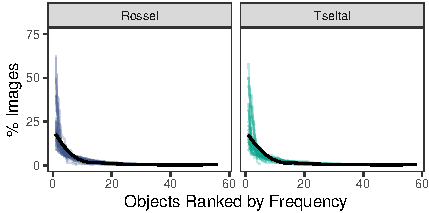
\includegraphics{figs/zipfian-objects-fig-1} 

}

\caption[Zipfian distribution of objects handled by each child across sites]{Zipfian distribution of objects handled by each child across sites. For each child, the top object was defined as the object appearing in the greatest number of images; thus, the identity of the top object does not match across all children.}\label{fig:zipfian-objects-fig}
\end{figure}
\end{CodeChunk}

Comparing across sites, 32.7\% of objects were present in both
communities, and several shared objects were among the most frequently
handled by children in both sites. In fact, among the top 25 most common
objects, 10 were shared across sites (Figure 3). Of note, the study
camera was the object that was handled by the most children in both
sites (Rossel: 69.2\%, Tseltal: 91.4\% of children). The camera and
other study-related objects (i.e., vest and privacy cover for the
camera), were retained in our analyses; however, inclusion of these
items did not qualitatively change any of the reported results.

\begin{CodeChunk}
\begin{figure*}[!ht]

{\centering 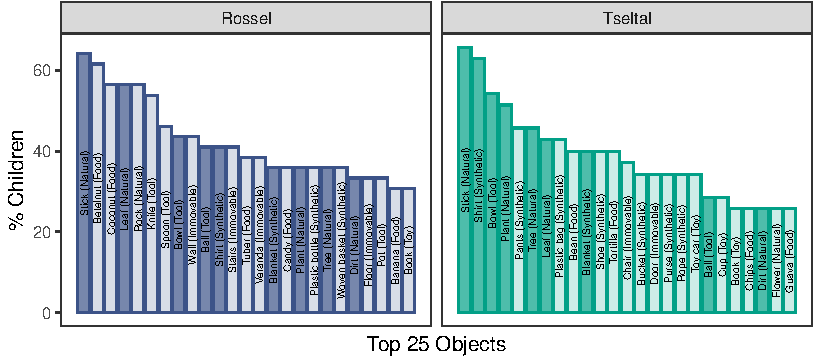
\includegraphics{figs/top-objects-fig-1} 

}

\caption[Non-study-related objects handled at least once by the most children in each site]{Non-study-related objects handled at least once by the most children in each site. Filled bars represent objects that were among the top 25 for both sites.}\label{fig:top-objects-fig}
\end{figure*}
\end{CodeChunk}

\hypertarget{effects-of-object-category}{%
\subsection{Effects of object
category}\label{effects-of-object-category}}

The frequency of object categories was similarly divided across sites
(Figure 4A). Children primarily handled food items
(\emph{M}\textsubscript{\emph{Rossel}} = 27.31\%,
\emph{M}\textsubscript{\emph{Tseltal}} = 31.52\% of handling) and
miscellaneous synthetic objects (e.g., rope, woven basket, bottle, etc.,
\emph{M}\textsubscript{\emph{Rossel}} = 24.3\%,
\emph{M}\textsubscript{\emph{Tseltal}} = 31.37\% of handling). For 51 of
75 children, their top category was either food or synthetic objects.
Two-tailed Wilcoxon tests revealed only one significant category-level
difference between sites: children's handling of large or immovable
objects, where Rossel children handled these objects more frequently
than Tseltal children (\emph{M}\textsubscript{\emph{Rossel}} = 10.79\%,
\emph{M}\textsubscript{\emph{Tseltal}} = 3.55\%, adjusted \emph{p} =
0.001, but these objects were still among the least frequently handled
in both sites. The initial predicted difference in synthetic object
handling between sites was significant; however, after correcting for
multiple comparisons, this effect did not persist (adjusted \emph{p} =
0.104).

\begin{CodeChunk}
\begin{figure}[!h]

{\centering 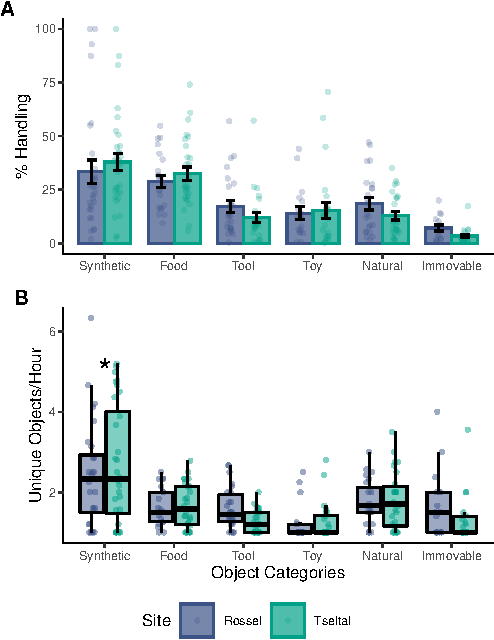
\includegraphics{figs/overall-stats-fig-1} 

}

\caption[(A) Overall frequency of handling by object category]{(A) Overall frequency of handling by object category. Points reflect percentages for individual children. (B) Count of unique objects handled per hour by object category. Points reflect means for individual children across all hours of recording. Asterisks indicate significant differences between sites after correcting for multiple comparisons.}\label{fig:overall-stats-fig}
\end{figure}
\end{CodeChunk}

During any given hour, children handled 6.5 objects from 3.66 different
categories, on average (median = 6 objects, \emph{SD} = 4.62, range =
1--27). To test for differences across sites and categories, we ran
individual linear mixed-effects models for each of the six object
categories, with category membership dummy coded (i.e., objects
belonging to the target category for a given model = 1, objects
belonging to other categories = 0). Models included fixed effects of
site, category, number of images, and site-by-category interaction as
well as random intercepts for individual children. After correcting for
multiple comparisons, we found a significant main effect of the
synthetic object category (\(\beta\) = 0.39, \emph{SE} = 0.09, \emph{t}
= 4.42, \emph{p} \textless{} 0.001) and a significant site-by-synthetic
interaction (\(\beta\) = 0.37, \emph{SE} = 0.12, \emph{t} = 2.98,
\emph{p} = 0.056) such that children handled more unique synthetic
objects per hour than objects from other categories, and this effect was
stronger for Tseltal children than for Rossel children. Additionally, we
found negative main effects for the toy (\(\beta\) = -0.45, \emph{SE} =
0.14, \emph{t} = -3.34, \emph{p} = 0.017) and work tool (\(\beta\) =
-0.73, \emph{SE} = 0.19, \emph{t} = -3.92, \emph{p} = 0.002) categories,
indicating that children handled fewer unique objects from these
categories per hour. Finally, a significant main effect of the immovable
object category (\(\beta\) = 0.46, \emph{SE} = 0.11, \emph{t} = 4.01,
\emph{p} = 0.001) and site-by-immovable interaction (\(\beta\) = -0.88,
\emph{SE} = 0.18, \emph{t} = -4.96, \emph{p} \textless{} 0.001) revealed
that children handled more unique immovable objects per hour than
objects from other categories, and this effect was stronger for Rossel
children than for Tseltal children (Figure 4B).

\hypertarget{effects-of-age}{%
\subsection{Effects of age}\label{effects-of-age}}

The frequency of object categories was largely stable over age (Figure
5). The only exception was a decreasing proportion of synthetic object
handling across developmental time for children in both sites (\(\beta\)
= -0.01, 0, \emph{SE} = 0, 0, \emph{t} = -2.28, -2.52, \emph{p} = 0.026,
0.014). {[}explain that this is driven by the fact that synthetic
objects are the most common and younger kids handle fewer objects{]}.
Thus, the broad composition of handled objects did not change
significantly as a function of age.

\begin{CodeChunk}
\begin{figure}[!ht]

{\centering 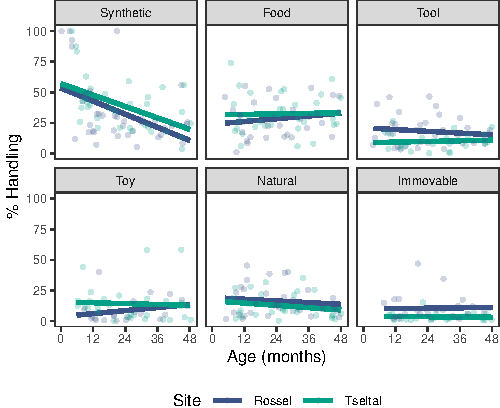
\includegraphics{figs/age-effects-bycategory-fig-1} 

}

\caption[Frequency of handling by object category across age]{Frequency of handling by object category across age. Individual points show raw percentages per hour for each child, and lines reflect model-predicted percentages.}\label{fig:age-effects-bycategory-fig}
\end{figure}
\end{CodeChunk}

However, children's overall \emph{rate} of object handling increased
significantly with age (Figure 6A). That is, older children handled more
unique objects per hour (\(\beta\) = 0.11, \emph{SE} = 0.03, \emph{t} =
3.18, \emph{p} = 0.002). Additionally, with increasing age, children
handled more objects from different categories per hour (Figure 6B;
\(\beta\) = 0.05, \emph{SE} = 0.01, \emph{t} = 4.14, \emph{p} = 0).
These effects were consistent across sites; we found no main effects of
site or interactions between site and age (all \emph{p}s \textgreater{}
0.05).

To further explore developmental changes in the characteristics of
children's object handling, we measured transitions between different
objects and different object categories. We modeled the relative number
of transitions per hour (i.e., number of transitions divided by the
number of possible objects or categories for the hour) as a function of
age and site, plus their interaction. We found no overall age-related
increase in object transitions (\(\beta\) = 0.01, \emph{SE} = 0,
\emph{t} = 1.43, \emph{p} = 0.157). However, there was a significant
main effect of site (\(\beta\) = -0.44, \emph{SE} = 0.14, \emph{t} =
-3.26, \emph{p} = 0.002) as well as a site-by-age interaction (\(\beta\)
= 0.01, \emph{SE} = 0, \emph{t} = 2.56, \emph{p} = 0.013) such that
Tseltal children made fewer transitions between objects per hour than
Rossel children but showed a steeper increase across age (Figure 6C). At
the category level, we found that, with increasing age, children made
significantly more transitions between object categories per hour
(\(\beta\) = 0.01, \emph{SE} = 0.01, \emph{t} = 1.77, \emph{p} = 0.08),
with no detectable differences across sites (Figure 6D).

\begin{CodeChunk}
\begin{figure}[!ht]

{\centering 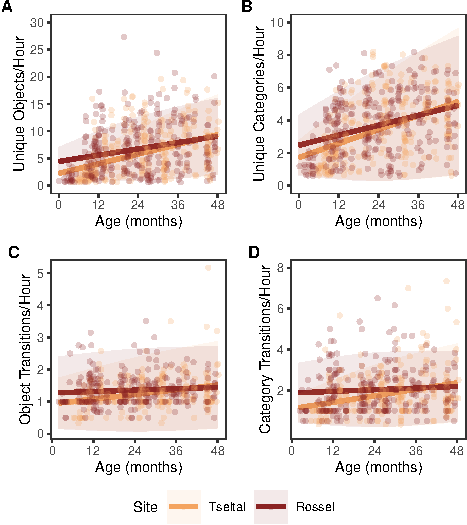
\includegraphics{figs/age-effects-fig-1} 

}

\caption[(A) Unique objects and (B) object categories handled per hour as a function of age]{(A) Unique objects and (B) object categories handled per hour as a function of age. (C) Relative number of transitions between objects and (D) object categories per hour as a function of age. Points reflect raw hourly counts for each child, and lines reflect model predictions with shaded standard error regions.}\label{fig:age-effects-fig}
\end{figure}
\end{CodeChunk}

\hypertarget{discussion}{%
\section{Discussion}\label{discussion}}

Just some miscellaneous notes for now

\hypertarget{cross-cultural-similarities-and-differences}{%
\subsection{Cross-cultural similarities and
differences}\label{cross-cultural-similarities-and-differences}}

Summary sentence of the broad overlap between communities on many of the
measures reported above, likely owing to the many characteristics that
are shared across these two cultural contexts (e.g., rural, swidden
horticulturalist, housed in multi-generation family complexes). However,
the differences that emerge between sites reveal the influence of market
integration, the organization of daily life, and infant carrying
practices (Brown \& Casillas, 2021; Casillas, Brown, \& Levinson, 2020,
2021; Casillas \& Elliott, 2021).

Marginally more unique synthetic objects for Tseltal children.
Discussion of the effects of market integration on the availability of
objects in Tenejapa vs.~Rossel Island.

More handling of large or immovable objects for Rossel kids. Discussion
of differences in the organization of young children's daily lives. More
time spent socializing on/near household verandas

Greater age-related increases in transitions between objects for Tseltal
children. Discussion of infant carrying practices. More time in sling
for Tseltal babies so fewer opportunities to seek out different objects
at the youngest ages.

\hypertarget{other-sources-of-consitency-and-variability}{%
\subsection{Other sources of consitency and
variability}\label{other-sources-of-consitency-and-variability}}

Possible changes with time of day and activity context as predicted in
prior work (e.g., morning mealtimes, Casillas, Brown, \& Levinson, 2020,
2021). Open question: are handled objects a good index for activity
context?

Changes from day to day: We don't know how much overlap there is from
day to day. While the exact objects may change, it's likely that they'd
follow a similar right-skewed distribution since we see this for most
kids in our sample and across mamy measures of children's input,
including visual (\textbf{clerkin2017real?};
\textbf{long2021characterizing?}) and linguistic
(\textbf{montag2018quantity?}).

Age: The broad composition of handled objects was largely stable across
age (consistent with \textbf{long2021characterizing?} for visually
present categories) but few categories here and also the possibility
that individual types may change. More here about manual dexterity and
possibly attention affecting object handling bout durations, which we
don't quantify here, but the transitions per hour analysis is a
first-pass way of (hopefully) getting at something similar

\hypertarget{consequences-for-learning}{%
\subsection{Consequences for learning}\label{consequences-for-learning}}

Zipfian distributions can be helpful for learning (e.g.,
\textbf{carvalho2019rethinking?}). Overlap between kids can get us to
start thinking about which object names and object-relevant words and
learned earlier. But important to note that there's less overlap between
kids (within sites) than we see for US context (e.g., Herzberg,
Fletcher, Schatz, \& Tamis-LeMonda, 2021), possibly owing to cultural
differences and sampling strategies (e.g., two-hour videos vs.~daylong
photos). Another point is that while there may be less overlap between
kids, there's likely more overlap between kids and adults (fewer
child-specific items)

Notes for near the end: Future plans to link to daylong audio
recordings. We can speculate about children's learning now that we have
some understanding of the distribution of object handling and the
identities of commonly handled objects. However, without knowing how
often children are also hearing \emph{talk} about the objects they're
handling, we can't fully address the word learning piece.

\hypertarget{references}{%
\section{References}\label{references}}

\setlength{\parindent}{-0.1in} 
\setlength{\leftskip}{0.125in}

\noindent

\hypertarget{refs}{}
\begin{CSLReferences}{1}{0}
\leavevmode\hypertarget{ref-adolph2010motor}{}%
Adolph, K. E., Karasik, L. B., \& Tamis-LeMonda, C. S. (2010). Motor
skill. In M. H. Bornstein (Ed.), \emph{Handbook of cultural
developmental science} (pp. 61--88). Psychology Press: New York, NY.

\leavevmode\hypertarget{ref-arnold2012life}{}%
Arnold, J. E., Graesch, A. P., Ochs, E., \& Ragazzini, E. (2012).
\emph{Life at home in the twenty-first century: 32 families open their
doors}. ISD LLC.

\leavevmode\hypertarget{ref-bergelson2019day}{}%
Bergelson, E., Amatuni, A., Dailey, S., Koorathota, S., \& Tor, S.
(2019). Day by day, hour by hour: Naturalistic language input to
infants. \emph{Developmental Science}, \emph{22}(1), e12715.

\leavevmode\hypertarget{ref-bergelson2017nature}{}%
Bergelson, E., \& Aslin, R. N. (2017). Nature and origins of the lexicon
in 6-mo-olds. \emph{Proceedings of the National Academy of Sciences},
\emph{114}(49), 12916--12921.

\leavevmode\hypertarget{ref-brownIPchildrearing}{}%
Brown, P., \& Casillas, M. (2021). \emph{Childrearing through social
interaction on {Rossel Island, PNG}}. (A. J. Fentiman \& M. Goody,
Eds.). New York, NY: Berghahn.

\leavevmode\hypertarget{ref-casey2022imco}{}%
Casey, K., Fisher, W., Tice, S. C., \& Casillas, M. (2022). ImCo: A
python tkinter application for coding lots of images (Version 2.0).
Retrieved from \url{https://github.com/kennedycasey/ImCo2}

\leavevmode\hypertarget{ref-casillas2020early}{}%
Casillas, M., Brown, P., \& Levinson, S. C. (2020). Early language
experience in a {Tseltal Mayan} village. \emph{Child Development},
\emph{91}(5), 1819--1835.

\leavevmode\hypertarget{ref-casillas2021early}{}%
Casillas, M., Brown, P., \& Levinson, S. C. (2021). Early language
experience in a papuan community. \emph{Journal of Child Language},
\emph{48}(4), 792--814.

\leavevmode\hypertarget{ref-casillasURdaylong}{}%
Casillas, M., \& Elliott, M. (2021). Cross-cultural differences in
children's object handling at home. PsyArXiv.
http://doi.org/\href{https://doi.org/10.31234/osf.io/43db8}{10.31234/osf.io/43db8}

\leavevmode\hypertarget{ref-fausey2016faces}{}%
Fausey, C. M., Jayaraman, S., \& Smith, L. B. (2016). From faces to
hands: Changing visual input in the first two years. \emph{Cognition},
\emph{152}, 101--107.

\leavevmode\hypertarget{ref-gaskins2000childrens}{}%
Gaskins, S. (2000). Children's daily activities in a {M}ayan village: A
culturally grounded description. \emph{Cross-Cultural Research},
\emph{34}(4), 375--389.

\leavevmode\hypertarget{ref-herzberg2021exuberant}{}%
Herzberg, O., Fletcher, K. K., Schatz, J. L., \& Tamis-LeMonda, C. S.
(2021). Infant exuberant object play at home: Immense amounts of
time-distributed, variable practice. \emph{Child Development},
\emph{XX}, 1--15.

\leavevmode\hypertarget{ref-jayaraman2017faces}{}%
Jayaraman, S., Fausey, C. M., \& Smith, L. B. (2017). Why are faces
denser in the visual experiences of younger than older infants?
\emph{Developmental Psychology}, \emph{53}(1), 38.

\leavevmode\hypertarget{ref-karasik2018not}{}%
Karasik, L. B., Schneider, J., Kuchirko, Y. A., \& Tamis-LeMonda, C. S.
(2018). Not so {WEIRD} object play in {T}ajikistan. Presentation to the
International Conference on Infant Studies, Philadelphia, PA.
http://doi.org/\href{https://doi.org/10.31234/osf.io/43db8}{10.31234/osf.io/43db8}

\leavevmode\hypertarget{ref-kretch2014crawling}{}%
Kretch, K. S., Franchak, J. M., \& Adolph, K. E. (2014). Crawling and
walking infants see the world differently. \emph{Child Development},
\emph{85}(4), 1503--1518.

\leavevmode\hypertarget{ref-laing2020babble}{}%
Laing, C., \& Bergelson, E. (2020). From babble to words: Infants' early
productions match words and objects in their environment.
\emph{Cognitive Psychology}, \emph{122}, 101308.

\leavevmode\hypertarget{ref-long2020detecting}{}%
Long, B., Kachergis, G., Agrawal, K., \& Frank, M. C. (2020).
\emph{Detecting social information in a dense database of infants'
natural visual experience}.

\leavevmode\hypertarget{ref-mcgillion2013supporting}{}%
McGillion, M. L., Herbert, J. S., Pine, J. M., Keren-Portnoy, T.,
Vihman, M. M., \& Matthews, D. E. (2013). Supporting early vocabulary
development: What sort of responsiveness matters? \emph{IEEE
Transactions on Autonomous Mental Development}, \emph{5}(3), 240--248.

\leavevmode\hypertarget{ref-sanchez2018detecting}{}%
Sanchez, A., Long, B., Kraus, A. M., \& Frank, M. C. (2018). Postural
developments modulate children's visual access to social information. In
\emph{Proceedings of the 40th annual conference of the cognitive science
society} (pp. 2412--2417).

\leavevmode\hypertarget{ref-super1976environmental}{}%
Super, C. M. (1976). Environmental effects on motor development: The
case of {`{A}frican infant precocity.'} \emph{Developmental Medicine \&
Child Neurology}, \emph{18}(5), 561--567.

\leavevmode\hypertarget{ref-yu2013joint}{}%
Yu, C., \& Smith, L. B. (2013). Joint attention without gaze following:
Human infants and their parents coordinate visual attention to objects
through eye-hand coordination. \emph{PloS One}, \emph{8}(11), e79659.

\leavevmode\hypertarget{ref-yurovsky2013statistical}{}%
Yurovsky, D., Smith, L. B., \& Yu, C. (2013). Statistical word learning
at scale: The baby's view is better. \emph{Developmental Science},
\emph{16}(6), 959--966.

\end{CSLReferences}

\bibliographystyle{apacite}


\end{document}
